\documentclass{article}

% Recommended, but optional, packages for figures and better typesetting:
\usepackage{microtype}
\usepackage{graphicx}
\usepackage{subfigure}
\usepackage{booktabs} % for professional tables
\usepackage{xcolor}
\usepackage{tikz}
% Corporate Design of the University of Tübingen
% Primary Colors
\definecolor{TUred}{RGB}{165,30,55}
\definecolor{TUgold}{RGB}{180,160,105}
\definecolor{TUdark}{RGB}{50,65,75}
\definecolor{TUgray}{RGB}{175,179,183}

% Secondary Colors
\definecolor{TUdarkblue}{RGB}{65,90,140}
\definecolor{TUblue}{RGB}{0,105,170}
\definecolor{TUlightblue}{RGB}{80,170,200}
\definecolor{TUlightgreen}{RGB}{130,185,160}
\definecolor{TUgreen}{RGB}{125,165,75}
\definecolor{TUdarkgreen}{RGB}{50,110,30}
\definecolor{TUocre}{RGB}{200,80,60}
\definecolor{TUviolet}{RGB}{175,110,150}
\definecolor{TUmauve}{RGB}{180,160,150}
\definecolor{TUbeige}{RGB}{215,180,105}
\definecolor{TUorange}{RGB}{210,150,0}
\definecolor{TUbrown}{RGB}{145,105,70}

% hyperref makes hyperlinks in the resulting PDF.
% If your build breaks (sometimes temporarily if a hyperlink spans a page)
% please comment out the following usepackage line and replace
% \usepackage{icml2023} with \usepackage[nohyperref]{icml2023} above.
\usepackage{hyperref}


% Attempt to make hyperref and algorithmic work together better:
\newcommand{\theHalgorithm}{\arabic{algorithm}}

\usepackage[accepted]{icml2023}

% For theorems and such
\usepackage{amsmath}
\usepackage{amssymb}
\usepackage{mathtools}
\usepackage{amsthm}

% if you use cleveref..
\usepackage[capitalize,noabbrev]{cleveref}

%%%%%%%%%%%%%%%%%%%%%%%%%%%%%%%%
% THEOREMS
%%%%%%%%%%%%%%%%%%%%%%%%%%%%%%%%
\theoremstyle{plain}
\newtheorem{theorem}{Theorem}[section]
\newtheorem{proposition}[theorem]{Proposition}
\newtheorem{lemma}[theorem]{Lemma}
\newtheorem{corollary}[theorem]{Corollary}
\theoremstyle{definition}
\newtheorem{definition}[theorem]{Definition}
\newtheorem{assumption}[theorem]{Assumption}
\theoremstyle{remark}
\newtheorem{remark}[theorem]{Remark}

% Todonotes is useful during development; simply uncomment the next line
%    and comment out the line below the next line to turn off comments
%\usepackage[disable,textsize=tiny]{todonotes}
\usepackage[textsize=tiny]{todonotes}

\newcommand{\D}{\text{d}}% leibniz notation d for derivatives/integrals
\renewcommand{\qed}{\hfill \ensuremath{\Box}}% white qed box aligned to the right
\newcommand{\lp}[1]{\left({#1}\right)}% large parentheses, e.g. for vectors or fractions
\newcommand{\mono}{\texttt}% monospace text
\newcommand{\ceil}[1]{\left\lceil{#1}\right\rceil}
\newcommand{\floor}[1]{\left\lfloor{#1}\right\rfloor}
\newcommand{\cont}{\lightning}

\icmltitlerunning{Project Report for Data Literacy 2023/24}

\begin{document}

\twocolumn[
\icmltitle{
    Project Report for Data Literacy 2023/24\\ 
    Grade Inflation in the German School System - Causes and Effects
}

\icmlsetsymbol{equal}{*}

\begin{icmlauthorlist}
\icmlauthor{Jonathan Schwab}{equal,first}
\icmlauthor{Lars Kasüschke}{equal,second}
\icmlauthor{Niklas Munkes}{equal,third}
\icmlauthor{Tom Freudenmann}{equal,fourth}
\end{icmlauthorlist}

\icmlaffiliation{first}{Matrikelnummer 6765897, jonathan.schwab@student.uni-tuebingen.de, MSc Computer Science}
\icmlaffiliation{second}{Matrikelnummer 4247775, lars.kasueschke@student.uni-tuebingen.de, BSc Computer Science}
\icmlaffiliation{third}{Matrikelnummer 4269436, niklas.munkes@student.uni-tuebingen.de, MSc Media Informatics}
\icmlaffiliation{fourth}{Matrikelnummer 6631101, tom.freudenmann@student.uni-tuebingen.de, MSc Computer Science}

\vskip 0.3in
]
\printAffiliationsAndNotice{\icmlEqualContribution}

The reasons for the increase in Abitur grades have been a highly discussed topic in German society. Often, the reason for this is attributed to grade inflation. In this paper, we will show why this is not the case. Student competence has increased. One of the most important factors is the student-teacher ratio. We will show that this metric has a high correlation with the Abitur grades.


\section{Introduction}
(Motivation)
The Abitur grades have constantly increased in the german school system over the past decades. Every year, when the Abitur takes place, the grades and the appropriateness of difficulty of exercises is the hot topic in media. \\
There is a high desire to criticize the german school system, political decisions and the comission responsible for conducting the exam. It is a fertile ground for loosely justified speculations. One thesis that comes up every year is that the Abitur is getting easier. (Zeitungartikel)\\\\
(Current research)
Is the thesis "the Abitur is getting easier" justified and can it be supported with data? It is really hard to supported that claim by looking at the exercises, since difficulty is not measurable and somewhat subjective. Math has been the main battleground of the discussion. There are multiple studies looking at specific exercises and comparing them to past exercises \cite{kuhnel2015modellierungskompetenz} \cite{JahnkeKleinKühnelSonarSpindler+2014+115+122} \cite{lemmermeyer2019zentralabitur}. For the reasons above, this approach is highly controversial. On the other side multiple papers also argue that the overall competence of students has been increased, so a grade deflation can not be proven \cite{Schleithoff+2015+3+26}\\ Other discussed reasons for grade inflation are Many are speculative. Still, the improving grades are probably caused by multiple factors.\\\\
In this paper we argue, that the justifications for the claim that the Abitur is getting easier over the years, are barely supported by actual data. The various arguments made are usually based on subjective opinions and experiences.
(Topic of the paper)
This paper examines claims regarding the factors contributing to the improvement of Abitur grades and inverstigates which of these claims are supported by the data. This data analysis provide an explanatory framework for the improvement of Abitur grades by analysing data mainly from the German Federal Statitical Office and other federal ressources.\\
Further we will investigate what the measurable effects of the increasing Abitur grades are and if those effects are positive or negative. Finally we will make a prediction for the grade development of the future and the future of the german school system.


%!TEX root = ../report_template.tex
\section{Methods}
%Todo: Introduction

\subsection{Mathematical Basics}
% Todo: Introduction 

% Todo: Linear Regression

The Pearson correlation coefficient \cite{rodgers_thirteen_1988}, denoted as $r$, is a statistical measure used to assess the linear relationship between two sets of data, $X$ and $Y$. It is computed as the ratio of the sample covariance of the $X$ and $Y$ to the product of their sample standard deviations:
\begin{equation}
    r = \frac{\sum_{i=1}^n (X_i - \overline{X}) (Y_i - \overline{Y})}{\sqrt{\sum_{i=1}^n(X_i-\overline{X})^2 \cdot \sum_{i=1}^n(Y_i-\overline{Y})^2}}
\end{equation}

\subsection{Datasets}
% Maybe move it later
\begin{figure*}[t!]
    \centering
    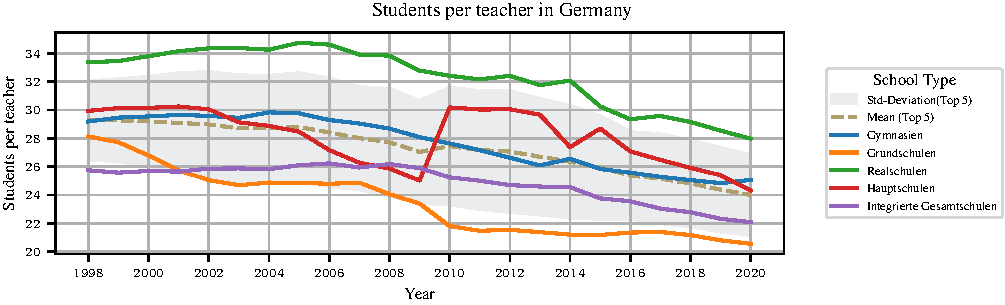
\includegraphics{fig/fig_students_per_teacher_per_school_type.pdf}
    \caption{Students-to-teacher ratio of the five most common school types in Germany. The ratio of full- and part-time teachers is displayed for each school type and aggregated to their mean (\textcolor{TUgold}{\rule[-0.2ex]{0.5em}{2pt} \rule[-0.2ex]{0.5em}{2pt}}) and standard deviation (\textcolor{TUgray}{\rule[-0.2ex]{1em}{0.8em}}).}
    \label{fig:spt-type}
\end{figure*}

This paper investigates both causes and effects of the phenomena discussed in \autoref{sec:Introduction}. Thus the analyzed datasets may be grouped by the information they represent into \emph{cause} and \emph{effect} datasets.

In the following, \emph{causes} shall be defined as the social, demographic and/or political factors that may influence the german school system such as the number of students, teachers, or budget provided by the German government. In contrast, \emph{effect} refers to the observable impact of these causes on any measure modelling the students' performance, e.g. average grades, PISA study results, or the rate of repeaters and school-leavers.

% Causes
The first cause dataset is the \textit{Fachreport Schuljahr 2020/21} of the \citeauthor{statistische_bundesamt_allgemeinbildende_2022} presenting the number of teachers from 1992 until 2020. The dataset groups them by their contract type, federal state, and school type. For the analysis, this paper merges the teacher counts with two student datasets, which are published in the \textit{Genesis} database provided by the \citeauthor{statistische_bundesamt_statistisches_2023}. These contain the number of children as different groupings and aggregations. The first (Table $21111-0002$) contains the number of children per grade and school type  for the years 1998 to 2022. In contrast, the second table (Table $21111-0010$) provides the absolute amount of children, leavers, and beginners in each federal state from 1997 to 2022. Therefore, the analysis of the merged dataset can only be conducted separately for school types and federal states.

Additionally, this paper considers the budget per child (Table $21711-0011$) as a possible cause which is provided in the \textit{Genesis} database of the \citeauthor{statistische_bundesamt_statistisches_2023}. The dataset contains the budget per child for the years 2010 to 2022 and is grouped by federal states. In contrast to the demographic and societal causes above, the budget can be regarded as a primarily political factor. To adjust for inflation, the budget is multiplied with the \textit{Verbraucherpreisindex} relative to 2022 provided by the \citeauthor{statistische_bundesamt_statistisches_2023}. 


% Effects
Moreover, the effects on students' performance are the basis for the analysis of the German school system, since they indicate whether the grade inflation exists or not. One of the few publicly available datasets containing grades is the average Abitur grades per federal state. The grades are published every year in a separate report by the \citeauthor{kultusminister_konferenz_abiturnoten_nodate}. Each file contains the count of children per written grade and federal state. In addition, the grades are given in $0.1$ steps, with $4.0$ as the worst and $1.0$ as the best grade. The amount of children who failed with a grade worse than $4.0$ is aggregated in an additional column. 

Although this is a great model for the performance of children attending grammar schools, a general performance measure for all school types is required to translate the results to all school types. Accordingly, this paper uses the number of repeaters (Table $21111-0014$) derived from the \textit{Genesis} Database of the \citeauthor{statistische_bundesamt_statistisches_2023}. There, the absolute count of repeaters by federal state, school type, and year is provided for the years 1998 to 2022.

% Say that also other effects such as people without degree, special educational needs were also explored but don't have a big impact due to their low percentage relative to all schoolchildren

\subsection{Exploratory Data Analysis}
% Todo: Better Introduction

Having introduced all used datasets, this paragraph aims to investigate potential patterns through an exploratory data analysis of the potential causes and effects. 

% Describe causes
% Todo: Sources
Firstly, regard the demographic effects on the number of children attending school and teachers employed by school type and federal state. The exploratory data analysis has shown that the number of schoolchildren decreases steadily from 1998 to 2014. Instead, it increased from 2019 to 2022 because more children started their education and fewer left school. Furthermore, more children graduate from grammar schools with university entrance qualifications. This demographic effect is combined with an increasing number of teachers across all German school types and federal states. Although, the percentage of part-time teachers is increasing, the number of full-time teachers is decreasing until 2020.

Given the hypothesis that having more teachers per student increases the quality of teaching, the datasets can be merged. As already explained, this merge can only been done separately for school types and federal states. Furthermore, the student-to-teacher ratio is calculated over all full- and part-time teachers, since they represent the majority ({\raise.17ex\hbox{$\scriptstyle\mathtt{\sim}$}} $90\%$) of the distribution. In contrast, the teachers who are employed on an hourly basis are excluded due to their small impact on the teaching quality and sparse representation in the data. The results (\autoref{fig:spt-type}) show that from 1998 to 2020, the ratio decreased for the five most common school types. As a result, the average decreases from 29 to 24 children per teacher. Together with the hypothesis, it follows that the quality of teaching should increase, and thus the performance measures should increase.

Besides the demographic measures, the budgets for the school system differ between the federal states. The analysis of the adjusted budget to inflation per child has shown that it steadily increases for all federal states. Although, this may be caused by the increasing number of teachers and the goals of digitalization of schools in the last years \cite{cone_pandemic_2022}.

% Effects

Now that the basic effects that may influence the students' performance have been identified, it is possible to study the performance measures. As the analysis of the students datasets has shown, more children are attending grammar schools in Germany. Thus, the average Abitur grade of the children is a great measure of the performance of many children. \autoref{fig:rising-grades} shows that the average grades are increasing in all federal states. Furthermore, a linear regression can be employed to represent their mean. Importantly, the regression is calculated on the data before 2021 because of the COVID-19 pandemic beginning in 2020. In 2022, the grades significantly increased compared to the years before the pandemic. This could indicate that the pandemic has had novel consequences for the educational system. Due to the lack of data following the pandemic, this paper will solely focus on the linear trend until 2020. Furthermore, an additional analysis of the relative number of failed students has shown that the failure rate has no repetitive or linear pattern. Therefore, the provided results in \autoref{fig:rising-grades} are only valid for children graduating with a grade of at least 4.0.

\begin{figure}[h]
    \centering
    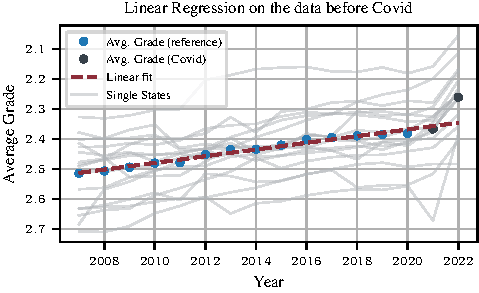
\includegraphics{fig/fig_rising_grades.pdf}
    \caption{Average Abitur grades before (\textcolor{TUlightblue}{\tikz\draw[fill={TUlightblue}] (0,0) circle (0.25em);}) and after the COVID-19 pandemic (\textcolor{TUdark}{\tikz\draw[fill={TUdark}] (0,0) circle (0.25em);}) with a linear regression line (\textcolor{TUred}{\rule[-0.2ex]{0.5em}{2pt} \rule[-0.2ex]{0.5em}{2pt}}) of the years 2007 to 2020. In the background the figure contains average grades foreach federal state (\textcolor{TUgray}{\rule[-0.2ex]{0.5em}{1pt}}).}
    \label{fig:rising-grades}
\end{figure}

Moreover, all children attending other schools have no direct impact on the results of the Abitur grades. Therefore, the number of repeaters per federal state, school type, grade, and school year is analyzed. To enhance the relevance of the results, the relative ratio of repeaters is calculated by dividing the absolute counts by the absolute number of schoolchildren. This results in an aggregation for the federal states per year and in one for the school types per year. As a result, the number of repeaters has decreased for all educational institutions and federal states from 1998 to 2020. Hence, the trend equals the expected result, after analyzing the Abitur grades.

To summarize, the exploratory findings indicate an increasing number of students and teachers, resulting in a decreasing ratio of students to teachers and a rise in the budget per child. The possible outcomes include a linear increase in Abitur grades in grammar schools and a shrinking proportion of repeaters in general.

% Todo: Move this into results --> adapt their on the argumentation
\paragraph{Correlation and Relationships}
The relationships can be explored by combining the datasets, plotting the interesting variables, and calculating the correlation coefficients between them. Since the student-to-teacher ratio aggregates the number of students and teachers, this section will correlate the other variables against it.

Therefore, the first  correlation exists between the average Abitur grade in Germany and the student-to-teacher ratio. Initially, the average grades across all federal states are calculated and then compared to the student-to-teacher coefficient for German grammar schools. As shown in \autoref{fig:regression-stt-grade} the relationship between both is nearly linear. In addition, the result contains neither clusters nor outliers. Hence, a smaller student-to-teacher ratio results in better grades. Additionally, the Pearson correlation value is $0.98$, indicating a strong positive correlation. This emphasizes the initial hypothesis and increases the importance of a good care factor between teachers and children.

\begin{figure}[h]
    \centering
    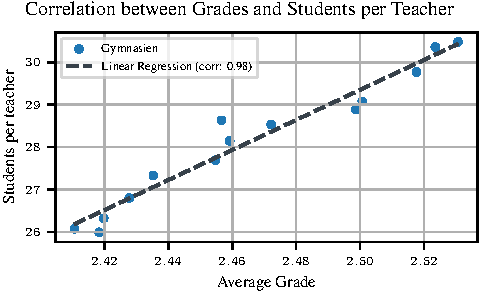
\includegraphics{fig/fig_correlation_grades_students_per_teacher.pdf}
    \caption{Linear regression on the students-to-teacher ratio by average Abitur grade. The resulting regression line (\textcolor{TUred}{\rule[-0.2ex]{0.5em}{2pt} \rule[-0.2ex]{0.5em}{2pt}}) is calculated over the aggregated average overall grammar schools (\textcolor{TUlightblue}{\tikz\draw[fill={TUlightblue}] (0,0) circle (0.25em);}) in Germany.}
    \label{fig:regression-stt-grade}
\end{figure}

As already explained, these results correspond only to grammar schools and are not necessarily representable for other schools or single federal states. Thus, the student-to-teacher ratio is also compared to the repeaters and the budgets per child in each federal state. Therefore, their Pearson correlation coefficients are calculated for each federal state across all years. 

\autoref{fig:heatmap_correlation_students_per_teacher_repeaters_budget} presents a visualization of the Pearson correlation coefficients, analyzing the relationship between the number of children per teacher and the average number of repeaters, as well as the educational budget per child. To visually represent the data across various federal states, a heatmap is generated. Therefore, the Pearson correlation coefficients for each state is normalized to the used color map scale. Consequently, each state is assigned a color representing the correlation coefficient. It is evident that there exists a strong positive correlation between the student-to-teacher ratio and the rate of repeaters in the most new federal states, while the correlation in the new federal states is significantly weaker. Moreover the correlation between the student-to-teacher ratio and the inflation adjusted budget per child tends to be positive for the new federal states and negative for the old federal states.

\begin{figure}[h]
    \centering
    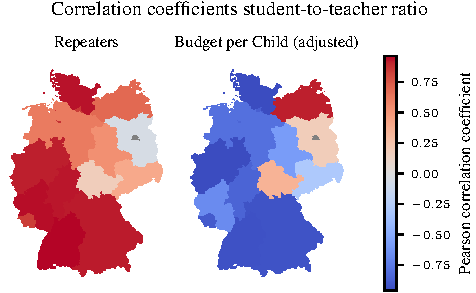
\includegraphics{fig/fig_heatmap_correlation_students_per_teacher_repeaters_budget.pdf}
    \caption{Pearson correlation coefficients between the student-to-teacher ratio and the relative repeater count (left) and the inflation-adjusted average budget per child (right). \textcolor{red}{Red} indicates positive, \textcolor{gray}{gray} neutral, and \textcolor{blue}{blue} negative correlations between the variables.}
    \label{fig:heatmap_correlation_students_per_teacher_repeaters_budget}
\end{figure}


\section*{Results}
The mostinteresting finding is the strong correlation between the students per teacher ratio and the Abitur grades. Intuitevly this makes sense, since more teacher should result in smaller class sizes and less stress for the teachers, which makes for a better learning experience. The correlation between education performance and availabilty of teaching personnel is not new to research \cite{doi:10.1080/00220485.1984.10845072}, but it was usually discussed in the context of university performance (Quelle). It is especially important, since the student teacher ratio got smaller over the current years and the grades went on a steep increase. This marks the importance of having enough teaching personnel for every school.\\\\
It would be easy to say that the schools just need more money, so they can employ more teachers, but that's not the whole story. In this case, thüringen, Sachsen-Anhalt and Brandenburg stand out. For them the correlation between budget and students per teacher is negative. This could be a classic case of the East-West-Gap in Germany. The exact reasons are up to speculation, but a plausible explanation might go like this: Schools get money mainly based on how many children they have -> If certain schools get more children, they might wanna employ more teachers -> Because they don't have enough teachers in these states, they can't -> Schools get more money, but the number of teachers stay the same: Negative correlation.\\\\
The same anomaly can be observed with the repeaters. Here, we think a different phenomenon is accountable for this. Schools in Thüringen and Sachsen-Anhalt rely more and more on Teilzeitkräfte. This means that the overall proportion of teachers increases, while the grades stay the same, or even worsen, becasue there is more flucuation in teaching presonell for a given class. Thus we get a negative correlation.\\\\
That said, we can observe that for every other of the 16 federal states there is a very strong positive correlation, not only between Abitur grades but also the number of repeaters decreases. This means that it not only leads to better grades, but the weak ones won't left behind if enough teachers are available. But money doesn't necessaraly help here. There need to be enough teachers available to employ. From this analysis we conclude that making sure that many teachers are avilable is one of the most important challenges for the education system. Especially because right now there is still more open positions, than teachers that can fill them. The prognosis of the german education minister conference (Kultusministerkonferenz) gives a positive outlook. Their forecast is, that this gap will close in the coming ten years. This means that we can expect a further increase in grades in the future\\\\
It is important to note, having enough teachers is not the only factor at play here. We have shown, that it is one of the most important ones. The german education system has a lot of problems, but as we have shown, it has been solving some of the in the last decade. To say it is just because a grade inflation is happening, as it is a very common argument made, is a simplification and might be entirely wrong. The increasing grades are a result of an increase in competence of the students, facilitated by an improve in the education system, especially a decrease in the student teacher ratio.\\\\


%!TEX root = ../report_template.tex
\section{Conclusion}
This exploratory data analysis found correlations between the ratio of students and teachers, Abitur grades, repeaters, and budget-per-child. These indicate the importance of employing enough teachers, to increase children's performances. Prognoses are  showing that there are still more open positions than teachers available \cite{kultusminister_konferenz_lehrkrafteeinstellungsbedarf_2023}. Fortunately, the \citeauthor{kultusminister_konferenz_lehrkrafteeinstellungsbedarf_2023} predicts that this gap will eventually close in the coming decade.

Furthermore, the absence of teachers has an influence on the Abitur grades. It is evident from the observed correlations that the grades should get worse in the short term and increase in the long term, if there are no other factors influencing the Abitur grades. All in all, this analysis shows that grades at schools do not only rise due to grade inflation, but are also influenced by other positive factors.

% It is important to note that having enough teachers is not the only factor responsible for the rising Abitur grades. Nonetheless, it is one of the most important ones. While the German education system faces several challenges, this analysis illustrates that it has effectively addressed certain issues over the past decade and is poised to continue resolving them in the future. The increasing grades are a result of an increase in the competence of the students, facilitated by an improvement in the education system, especially a decrease in the student-teacher ratio.

% We have introduced a new approach to explaining the increasing Abitur grades. There is a strong correlation between the student-teacher ratio and the Abitur grades. Additionally, we also found a negative correlation between this ratio and the repeater number. This means that the number of teachers not only has a positive impact on the grades but also on the more challenged students. Improving the budget does not necessarily help. It is essential for the German education system to have enough teachers available.

% Todo Reuse 
% Grade inflation in the Abitur grades has not been scientifically proven so far. What has been proven is that student competence is increasing. It is important to acknowledge that the student-teacher ratio is not the only factor at play in improving education and, thus, student competence. Multiple factors are at play; some are already known through research, and some still need to be discovered. We have shown that the student-teacher ratio is a crucial one.


\bibliography{bibliography}
\bibliographystyle{icml2023}

\end{document}
